\documentclass[a4paper]{article}

\usepackage{fullpage} % Package to use full page
\usepackage{parskip} % Package to tweak paragraph skipping
\usepackage{tikz} % Package for drawing
\usepackage{amsmath}
\usepackage{hyperref}
\usepackage{enumitem}
\usepackage{mathtools}
\usepackage{graphicx}
\usepackage{listings}

\title{Scalable Machine Learning - Review Questions 6}
\author{TheBrightSideOfLife: Giorgio Ruffa - Erik Wouters}
\date{11/12/2018}

\begin{document}

\maketitle

\url{https://id2223kth.github.io/slides/questions6.pdf}

\section{CNN Parameters}
Using \texttt{SAME} padding implies that on the $x$ and $y$ axes there will be a row of zero's added at $x=-1 \cup y=-1$. Also there will be enough zeros added to the other end of $x$ and $y$ such that the middle of the filter can reach the last pixels of $x$ and $y$.


As we are dealing with RGB images the lowest convolutional layer has $200 \times 3 = 1200$ inputs and $400$ outputs. For each of the outputs there is also a bias. The filter size is $3 \times 3$. This makes $(3 \times 3 \times 18000 + 1) \times 400$ parameters for that layer.

NOT SURE, NEEDS TO BE FIXED


\section{CNN filter}
If we apply the filter in the on the right of figure \ref{fig:q2} to the image on the left using a stride of $2$ in both the $x$ and $y$ directions we get the filtered image in \ref{mat:ans}.

\begin{figure}[ht]
  \centering
  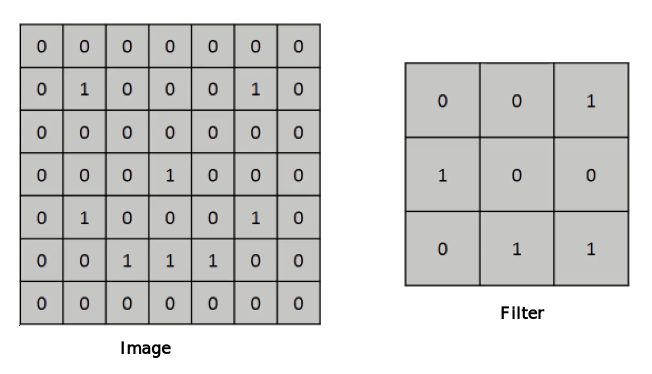
\includegraphics[scale=0.4]{Reports/Images/q2.png}
  \caption{Image and Filter}
  \label{fig:q2}
\end{figure}

\begin{align}
\begin{bmatrix}
     0              & 0             & 0             \\
     \frac{1}{9}    & 0             & \frac{1}{9}   \\
     0              & \frac{1}{9}   & \frac{1}{9}   \\
 \end{bmatrix}
 \label{mat:ans}
\end{align}

The following Python code snipped can be used to compute the result of the filter:

\begin{lstlisting}[language=Python]
def cf(im, filt, stride=1):
    nx = int(np.ceil((im.shape[0] - filt.shape[0] + 1) / stride))
    ny = int(np.ceil((im.shape[1] - filt.shape[1] + 1) / stride))
    image = np.zeros(shape=(nx, ny))
    for x in range(nx):
        for y in range(ny):
            image[x, y] = np.sum(
                im[
                    x * stride : x * stride + filt.shape[0],
                    y * stride : y * stride + filt.shape[1],
                ]
                * filt
            )
    return image / np.prod(filt.shape)
\end{lstlisting}


\section{Accuracy}
The correct answer is (c). When the number of kernels increases above a certain limit (which depends on the variance of the input image) the correlation between the kernels starts to increase. This does indeed help the model to overfit the data.

% \bibliography{bibliography}{}
% \bibliographystyle{plain}

\end{document}